\documentclass[12pt]{article}
\usepackage{graphicx}
\usepackage[utf8]{inputenc}
\usepackage{xcolor}
\usepackage{hyperref}
\usepackage{float}
\usepackage[english]{babel}
\usepackage{fancyhdr}
\usepackage{longtable}
\usepackage{wrapfig}

\usepackage{listings}


 \usepackage{pdfpages}
 
 

\usepackage{amssymb,amsmath}

\usepackage{array,multirow}

\newcommand{\defi}{\stackrel{\triangle}{=}}







\newtheorem{definition}{Definition}[section]
\newtheorem{proposition}[definition]{Proposition}
\newtheorem{lemma}[definition]{Lemma}
\newtheorem{corollary}[definition]{Corollary}
\newtheorem{theorem}[definition]{Theorem}
\newtheorem{claim}{Claim}[definition]
\newtheorem{note}[definition]{Note}




 
 

\addtolength{\headheight}{1.5cm} % make more space for the header
\pagestyle{fancyplain} % use fancy for all pages except chapter start
\lhead{
\includegraphics[height=0.1cm]{Images/logo_hidden.png}} % left logo
\rhead{
\includegraphics[height=2.3cm]{Images/logo.png}} % right logo
\renewcommand{\headrulewidth}{0pt} % remove rule below header



\begin{document}




\begin{titlepage}

\newcommand{\HRule}{\rule{\linewidth}{0.5mm}} % Defines a new command for the horizontal lines, change thickness here

\center % Center everything on the page
 
%----------------------------------------------------------------------------------------
%	HEADING SECTIONS
%----------------------------------------------------------------------------------------

\textsc{\LARGE Università La Sapienza}\\[1.5cm] % Name of your university/college
\textsc{\Large Facoltà di Ingegneria dell’Informazione, Informatica e Statistica}\\[0.5cm] % Major heading such as course name
\textsc{\large Dipartimento di Informatica}\\[0.5cm] % Minor heading such as course title

%----------------------------------------------------------------------------------------
%	TITLE SECTION
%----------------------------------------------------------------------------------------

\HRule \\[0.4cm]
{ \huge \bfseries Method to Recognize Greenpass}\\[0.4cm] % Title of your document
\HRule \\[1.5cm]
 
%----------------------------------------------------------------------------------------
%	AUTHOR SECTION
%----------------------------------------------------------------------------------------

\begin{minipage}{0.4\textwidth}
\begin{flushleft} \large
\emph{Author:}\\
Giordano \textsc{Dionisi}

\end{flushleft}
\end{minipage}
~
\begin{minipage}{0.4\textwidth}
\begin{flushright} \large
\emph{Supervisor:} \\
Prof. Maria \textsc{De Marsico} % Supervisor's Name
\end{flushright}
\end{minipage}\\[2cm]

% If you don't want a supervisor, uncomment the two lines below and remove the section above
%\Large \emph{Author:}\\
%John \textsc{Smith}\\[3cm] % Your name

%----------------------------------------------------------------------------------------
%	DATE SECTION
%----------------------------------------------------------------------------------------

{\large \today}\\[2cm] % Date, change the \today to a set date if you want to be precise

%----------------------------------------------------------------------------------------
%	LOGO SECTION
%----------------------------------------------------------------------------------------












%%%%%%%%%%%%%%%%%%%%%%%%%%%%%%%%%%%%%%%%%%%%% COOL IF IS ADDED

%%
\includegraphics{Images/logo_firstpage.png}\\[1cm] % Include a department/university logo - this will require the graphicx package

%%%%%%%%%%%%%%%%%%%%%%%%%%%%%%%%%%%%%%%%%%%%%








%----------------------------------------------------------------------------------------

\vfill % Fill the rest of the page with whitespace


\end{titlepage}


\newpage
\tableofcontents
\newpage


\section{Introduction}

    Research problem 5: Extracting a distinct and
    portable “signature” of a subject from the data gener-
    ated by the built-in sensors present in smartphones and
    wearable devices.

    -- Bello e fattibile ... noi abbiamo già lavorato su gait catturato da accelerometro e handwriting usando lo smartphone nell'aria --


Capire come sfruttare tali metodi di riconoscimento o migliorare gli esistenti  -- LO ACCETTEREI CON RISERVA PER LA DIFFICOLTÀ

A portable signature is a method to authenticate a specific person. This is a clever method because in this way we can have the possibility to take always with us the authentication method. Also in this way this signature consists of an evaluation and an sense of all the environment around a specific person to authenticate. In fact we use the several sensors in our smartphone to keep track of our movements and to see if a specific person is a right person or not.

So we can obtain a portable signature by means of the sensors of a wearable device, such as the smartphone.

For this reason, first of all, it's important know the amount of sensors that we have in an wearable device, like as a smartphone. We have many sensors, namely:

\begin{enumerate}

\item Accelerometer: An accelerometer detects acceleration, vibration, and tilt to determine movement and exact orientation along the three axes. Apps use this smartphone sensor to determine whether your phone is in portrait or landscape orientation.

It can also tell if your phone screen is facing upward or downward. The accelerometer can also detect how fast your phone is moving in any linear direction.

\item Gyroscope: Gyroscope also provides orientation details and direction like up/down and left/right but with greater precision like how much the device is tilted. This is where it differs from accelerometer — gyroscope can measure rotation too but the former cannot.

So it can tell how much a smartphone has been rotated and in which direction. Popular apps like Pokemon Go and Google Sky Map use gyroscope sensor to determine the direction towards which our phone is pointed.

\item Magnetometer: Our smartphones are equipped with magnetometer which we commonly recognize as a compass. It can detect magnetic fields, so the compass app in phones uses this smartphone sensor to point at the planet’s north pole.

Whenever you open Google Maps or Apple Maps, the magnetometer is fired up to determine which way the map should be. This sensor can detect metal very well, so it is used in metal detector apps too.

    The absolute orientation of a phone is represented in angles yaw, pitch, and roll. It is detected by a combination of the accelerometer, compass, and gyroscope.

\item GPS: Global Positioning System (GPS) units in smartphone communicate with the satellites to determine our precise location on Earth. The GPS technology doesn’t actually use internet data this is why we can find our location on maps even after losing the signals, but the map itself is blurry as it requires internet to load the details — this is how offline map works. GPS is used in all location-based apps like Uber and Google Maps.

    The accelerometer, gyroscope, magnetometer, and GPS work together to create the perfect navigation system in your smartphone.

\item Proximity Sensor: A proximity sensor makes use of an infrared LED and IR light detector to find out how close the phone is to an outside object. It used while making calls and when the phone is held to the face to make or receive a call, the sensor detects it and disables the touchscreen display to avoid unintended input through the skin.

\item Ambient Light Sensor: The light sensor detects the lighting levels in the vicinity to adjust the display brightness accordingly. It is used in Automatic Brightness Adjuster to decrease or increase the brightness of the smartphone screen based on the availability of light.

\item Microphone: The microphone is basically a sound sensor that detects and measures the loudness of sound. While there are different types of microphone sensors available, smartphones generally use micro-sized electret microphones.

Apart from making and receiving calls, it is used for voice search and voice commands for digital assistant apps like Google Assistant, Siri, Cortana, etc.

\item Touchscreen Sensors smartphone sensors in a touchscreen have an electrical current passing through them at all times and touching the screen causes a change in the signals. This change acts as input for the device. Before Apple introduced the capacitive touchscreen, resistive screens were used in the display. But nowadays, the capacitive screen is used in almost all smartphones.

\item Fingerprint Sensor: Gone are the days of memorizing passwords and patterns to unlock your phone as many users prefer using the fingerprint scanner these days. Fingerprint sensor enables biometric verification to secure many smartphones today. It is a capacitive scanner that records your fingerprint electrically.

When you put your finger on its surface, the ridges in your fingerprints touch the surface whereas the hollows between the ridges have a slight separation. In short, it measures the varying distances and pattern between the ridges on the surface of your finger. This smartphone sensor is quite useful in apps that require authentication such as mobile payment apps.

    Also Read: How Does A Fingerprint Scanner Work — The Application Of Biometrics

\item Pedometer: The pedometer is used for counting steps, and fitness tracker makes use of this sensor to count the number of steps you take. Pedometers generally use the values generated by the accelerometer to monitor your movements like running or walking.

\item Barcode/QR Code sensors: Most of the smartphones have barcode sensors that can read a barcode by detecting the reflected light from the code. It generates an analog signal with varying voltage that represents the barcode. This analog signal is then converted to a digital one and finally decoded to reveal the information in it. Barcode sensors are useful in scanning the barcodes products or QR codes.

\item Barometer: There are many high-end Android phones like Pixel and iPhones that include a barometer in their hardware. The barometer measures the air pressure, so it is quite useful in detecting weather changes and in calculating the altitude you’re at.

\item Heart Rate Sensor: Next up is the heart rate sensor that measures heartbeat with the help of LED and optical sensors. The LED emits light towards the skin, and this smartphone sensor looks for the light waves reflected by it.

There is a difference in the light intensity when there is a pulse. The heartbeat is measured by counting the changes in light intensity between the minute pulsations of the blood vessels. Many fitness and health apps use this method to calculate the heart rate.4

\item Thermometer: Every smartphone comes with an inbuilt thermometer for monitoring the temperature inside the device and battery. In case a component starts overheating, the system shuts down itself to prevent any damage.

However, some handsets come with additional thermometers to measure ambient temperature. If you can recall, the Samsung Galaxy S4 bragged of thermometer that can measure temperature. Such thermometer sensors can be used by apps to detect your room temperature.

\item Air Humidity Sensor: Now that we are talking about Galaxy S4 let’s discuss the Air Humidity sensor as well. S4 was the first smartphone to incorporate an air humidity sensor. It could measure the humidity in the air, and the data collected by it would tell the user whether the given air temperature and humidity are optimum or not. But again, this type of sensor is used by selected handsets only.

\item Geiger Counter: Now, this is one smartphone sensor that you should not expect to find in common devices. In fact, there is only one phone that supports it – the Sharp Pantone 5. This handset has been released in Japan only. The Geiger Counter in it can measure the current radiation level in the area.

\item Camera: It is used to do photos, videos or to do face recognition (MAYBE TO UPGRADE)

\end{enumerate}

Now we can know that with the accelerometer we can authenticate persons. It's important remember that we often work in a closed-set, because it's impossible to enroll all persons in the world. So it can be important to understand (in a city, in a place, in a office and so on) who are specific persons. In fact we can use this portable signature to verify the identity claimed by a person, but it can be also possible to identify in a city how is a specific person, if it is a terrorist or a common person.
Now we can refer to the actual period. We see that we must have in some places a dedicated person that verify if a person has or hasn't the greenpass. If we think about it, it's simple think that this is a very expensive activity, in economic terms. We can do some examples:

\begin{itemize}

\item In University: We have a lot of people in university and mainly the controls aren't perfect, because if we have only a controller (for economic reason) and 1200 students, it's impossible to think that the controls are made perfectly for each student (this require a lot a lot of time really). Also if we have too many students we must have a student or a person that he checks greenpass for each person. This means that each person every day must give (to the controller) him certificate and this is a really time-consuming activity. It is also very boring to present every day same certificate and this isn't a lot acceptance for the persons

\item In Restaurant, Gym,...: Same problem than the precedent point. In fact we must check all certificates, but we know that activities haven't too much time, so frequently this controls aren't made well

\end{itemize}

It's also important remember that only authorities (like as Police and so on) can really verify if the claimed certificate is the correlated certificate of the person. In fact i't also possible that a person X present the greenpass of the person Y. Now X can access to all services, because the controller can't verify if the greenpass presented by the person X is really him greenpass

Instead we can have an application in the smartphones that can work like as a TAG (Autonomous Networking, RFID), namely the app sends a signal continuously (a bluetooth signal, a Wifi signal, a radio signal and so on) and when a reader reads this signal can verify if the specified person has the greenpass or not.

With this method we haven't the problem of camouflage, in fact we have a wearable device that it doesn't send its information, but it captures biometric information (like as with accelerometer) of the person and send them. So the reader doesn't authenticate the wearable device, but it authenticate the person by means of the wearable device. So this is a method more cheaper, because everyone has a wearable device with simple sensors, such as a smartphone (people that haven't a smartphone, like as old people, can show only the greenpass with the traditional method or they can use smartphone of another person) and the activities have to install only a tradictional reader of waves. This reader launch an error when a person hasn't greenpass (ring, for example) or it opens doors only when specified people have greenpass

This reader can only send queries to a distributed database (a centralized database for all these queries is impossible to think in 2021 !!) and this DB answers always to the reader. We can suppose that the DB tells "ALLOW" or "DENY" to the reader and this reply message is important. In fact if we think for a DB that reply only if there is any problem (so if the reader hasn't a reply it consider "ALLOW" message), then we can lose message in the channel, so we can admit person that haven't greenpass (False Acceptance). At the contrary if we have a system that reply only if a person is admitable (so if the reader hasn't a reply it consider "DENY" message), then we can lose the message in the channel and we cannot admit persons that have the greenpass. This persons must retry the access and this isn't confortable for them (remember that this new system has the main goal to be more accessible and acceptable for users, not to be frustrating).

So we have a reader, a sender, a DDB (Distributed DataBase of greenpass) and stop, no other people or systems.

But it's now important think about the sensor (or sensors) to use in this system to do the authentication. First of all it's important have a sensor that read biometric informations that are the most possible unique for each person. For this purpose it's important remember that prof. De Marsico has done a work on it. She has discovered that gait recognition is unique (statistically) and we can recognize people by means of it. It's simple to do because sensors (such as the accelerometer) in smartphone capture and analyse biometric informations of the person. These measurements are captured by an app installed on the smartphone that it has to only send these captured informations to the environment. People walk without problems and then reader reads this waves, decodes them and sends query to DDB. After It sees the reply of DDB and decides what to do with a specific person.

But in general it's important take, one by one, the sensors of smartphone and think on what of them is useless to authentication. In fact we remember that a biometric trait must be:

\begin{enumerate}

\item UNIQUE
\item ACCEPTABILITY
\item UNIVERSALITY
\item PERMANENCE
\item COLLECTABILITY

\end{enumerate}

Let's analyse each sensor and the biometric characteristics that it can read:

\begin{enumerate}
  \setcounter{enumi}{2}
  \item Magnetometer: It recognize an important feature, namely the feature of recognizing the north pole, so for an orientation purpose. Obviously our orientation isn't a biometric trait, because it is:
    \begin{enumerate}
    \item Not Unique --> Two different person, also in same time, can be oriented at the same point
    \item Not Permanence --> Usually persons move, so their orientation easily change with time
    \end{enumerate}
    So this isn't a biometric traits

    \item GPS: It analyse our position, but obviusly there are many problems, because if we authenticate a person by means of him position, then we have:
    \begin{enumerate}
    
    \item Not Unique --> Two different persons, in different times, can stay at the exactly same place and one can have the greenpass, while the other cannot have it
    \item Not Permanece --> Person usually moves, so how we can authenticate him if he change location?
    \end{enumerate}
    So also this sensor is totally useless for biometric purposes
    
    \item Proximity Sensor: With this sensor we donì't measure anything for a biometric trait. In fact we only measure the distance from the phone and us, but this isn't a useful characteristic, obviously

    \item Ambient Light Sensor: This sensor has a main problem -> It sees the light of the ambient, but we can tell that it can see our light. But in this case problems are:
    
    \begin{enumerate}
    
    \item Not Unique --> Two different persons can have same light, but one can have greenpass and other one cannot have greenpass
    \item Not Permanence --> Obviosly our light (that it should be better defined) can change with time
    
    \end{enumerate}
    
    So this isn't an interesting biometric characteristic, so we can discard it
    \end{enumerate}

\begin{enumerate}
  \setcounter{enumi}{7}
    
    \item Touchscreen Sensors: They only measure if there is a pressure from our fingers and the screen, but not other. So we can't authenticate anyone by means of only the knowledge of touching the screen or not..

\end{enumerate}
    
\begin{enumerate}
  \setcounter{enumi}{10}
    \item Barcode/QR Code sensors: This sensor is totally useless for our purposes; in fact we can use it to authenticate an object, but in biometry we authenticate something of person, not normally things (so we authenticate things of persons, namely)

    \item Barometer: A cool sensor that measure air pressure and characteristics of the behaviour. But this isn't interesting for a biometric point of view, because it doesn't measure anything for a person

    \item Heart Rate Sensor: This sensor has a lot of problems:
    
    \begin{enumerate}
    
    \item Not Universality --> Not every smartphone has this installed sensor
    \item Not Unique --> Two different persons can have same heart rate, but one can have greenpass and other one cannot have greenpass
    \item Not Permanence --> This isn't a characteristic that it doesn't change with time, in fact maybe a person that he runs and after goes to restaurant can have a high heart rate, but this doesn't imply that it hasn't greenpass, for trivial example
    
    \end{enumerate}
    
It is Collectability and acceptability, but this isn't enough for a good biometric trait (this sensor measures a not good biometric trait for biometrics purposes)

    \item Thermometer: This sensor isn't universal (by definition not every smartphone has an environment thermometer) and it measures the inside temperature of smartphone. Also if it measures temperature outside smartphone (like as the person temperature) we haven't uniqueness (same temperature is for different persons), universality (not every smartphone has external sensor of temperature), permanence (internal temperature of a person can easily change with the time). It is only acceptance (because sensor measures only a temperature) and collectability (it isn't difficult to measure temperature of a behaviour or of a person). It is cool discover this thing: at the beginning of the pandemy we have a person in activities that it measures temperature of each person: if there isn't the problem of universality, we could think to have a system like this to see, without a phisic person, which persons has fever and which haven't it. With the same system of a sender and a receiver (it isn't necesssary a DDB obviously).

    \item Air Humidity Sensor: Obviously this sensor not recognize some biometric features of person, but only features of the envoronment. So by definition it isn't really a biometric feature

    \item Geiger Counter: It measures radiations of environment and only one smartphone has this sensor. Obviously it doesn't measure feautures of persons and it isn't neither universal (only one smartphone in world has this sensor)

\end{enumerate}

So it's better recap the last sensors to treat:

\begin{enumerate}
    \item Accelerometer

    \item Gyroscope

\end{enumerate}
    
\begin{enumerate}
  \setcounter{enumi}{6}
  \item Microphone

\end{enumerate}

\begin{enumerate}
  \setcounter{enumi}{8}
  \item Fingerprint Sensor
  \item Pedometer

\end{enumerate}

\begin{enumerate}
  \setcounter{enumi}{16}
  \item Camera
  
\end{enumerate}

All of these sensors can authenticate persons: In fact we can use Accelerometer, Gyroscope and Pedometer together for gait recognition, the microphone for voice recognition and the fingerprint sensor for the finger recognition

We have supposed to use the gait recognition (it is very interesting) 9) (HERE) and we can suppose to use the fingerprint sensor only when the biometric system for gait recognition has some problems to recognize and authenticate a person or when we haven't too much space to do a good gait recognition (if it's necessary a lot of space) and so the simpler method can be the method of fingerprint. In this case people open their app when they are close to the reader, use the fingerprint sensor with their fingers and, in this way, the smartphone sends a signal to the reader to tell how the finger is formed. The reader query to DDB the identity of this finger and waits the answer. But this approach has some problems: in fact the smartphone cannot send to the reader the identity of the person for this finger, because we can memorize the finger of a person Y (without greenpass) and tell to the smartphone that there finger is of a person X (with greenpass). In this case smartphone sends to reader the identity of the X and reader query to DDB that it accepts, obviously, the person, but this is a wrong way --> Remember that the smartphone doesn't tell the identity supposed of a person, but it only tells data registered with its sensors. Obviously this approach is possible in countries like as United States, because there we have a DDB with all fingerprints of the persons, but in countries like as Italy this Database with fingerprints of all persons there isn't. So we must require to record finger when a person gets greenpass (with vaccine, healing or swab) and in this case the system doesn't see the identity, but it just sees if the finger memorized is in the DDB or not, it isn't necessary to link the registered finger in enrollment phase to an identity (it's only necessary memorize all fingerprints of greenpass' persons and the expiration date for each fingerprints). This is another possible way to authenticate persons, but this is only an alternative, it isn't our initial idea

\begin{enumerate}
  \setcounter{enumi}{6}
  \item For the microphone we have the voice recognition, but we can't suppose that we always work in noising enviroments (like as entrance of universities, restaurants, offices and so on), so we have to suppose to install a room without any noise, but this is expensive and people must talk. This requires time and the voice isn't a really unique characteristic, because isn't to much difficult to camouflage it. For this reason we discard it very easily
\end{enumerate}

\begin{enumerate}
  \setcounter{enumi}{16}
  \item With camera we can do the face recognition. 1-2-10) Our idea is to combine face recognition and gait recognition to authenticate persons. It isn't important know their identities, but DDB must have only faces and gaits, without an associated identity, only an expiration date. In this way we can see if the gait and/or face is in the DDB or not. In this way we can authorize or not persons that they want to enter in a specific place. The problem is that the camera should be installed on the reader, because if the person must stop to do face recognition with him smartphone, this can be not more acceptable and, also, this doesn't simplify the system, like as our initial idea. But a reader with this idea is a little more expensive and in enrollment phase (when we do swab, vaccine and so on) we must enroll also the face, over and above the gait. But it can be interesting to combine all of these features

\end{enumerate}

In this way we have a main gait recognition, after an eventual face recognition and, if there are problems, a fingerprint recognition. It's a faster system that we want to explain a lot in the following

But an important thing this: we are thinking to use a gait recognition system to avoid problems of greenpass' checks; but there is an enormous problem, namely the place where we have to do this recognition. In fact it's easy know that a normal restaurant or bar hasn't a large entrance where it's possible to take enough informations on gait of the persons (it's necessary around 10 meters for a good gait recognition)
This isn't, unfortunately, a solvable problem because we can't think to reserve a place enough large to see perfectly the gait of a person, because it isn't practical for money and space reasons and every gait recognition systems need at least few meters to capture the gait: so there are too many constraints
But we can do a similar idea, namely we can exploit the other possible sensors of smartphone, mainly camera. In fact we can do face recognition and the way is very easy:

\begin{enumerate}

\item Tom wants to enter in Gio's Brothers Pub

\item When Tom is at entrance he takes him phone and it opens our application

\item He shows his face to app and, then, the app sends a broadcast signal
\item Reader captures this signal and it sees in DDB: If face is in DDB (it isn't necessary to know identity), then Tom is authorized, otherwise he isn't authorized

\end{enumerate}

It's obviously possible think that reader has camera and it can recognize each person, but this can be very expensive according to the fact that restaurant, pub and so on have spent a lot of money in this long period to adapt them to the italian normatives
Obviously face recognition can't be perfect and the recognition can't be done: so we can have a multimodal system that it can do face recognition or fingerprint recognition to authorize persons
obviusly one of these must be mandatory when a person do the vaccine and so on; so we choose to have face recognition mandatory for the enrollment phase (it's more acceptability for users and more user-friendly for authentication, considering that this is a system that a person can use a lot a lot of times). Obviously fingerprint enrollment is recommended if face recognition has problems to recognize a certain person. It's important remember that there is also the last alternative for persons that they don't want to enroll face and so on, namely the original greenpass card or qr code for this purpose.

It's important consider a thing: we want have less possible value of false acceptance, namely number of wrong persons authorized must be slower as possible, because we want avoid that persons without greenpass can enter in a building: this can be possible on face recognition, after we have also other two ways to authenticate or not persons and we can have a fewer rigit threshold for fingerprint recognition, but always with a FAR (false acceptance rate) less possible

\begin{figure}[H]
    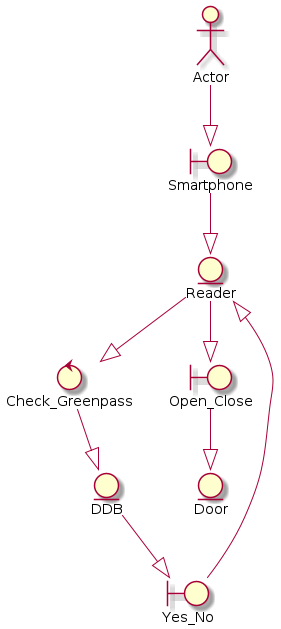
\includegraphics[width=\textwidth,height=\textheight,keepaspectratio]{./Images/System_Draw.png}
    \label{47_1}
\end{figure}

\begin{figure}[H]
    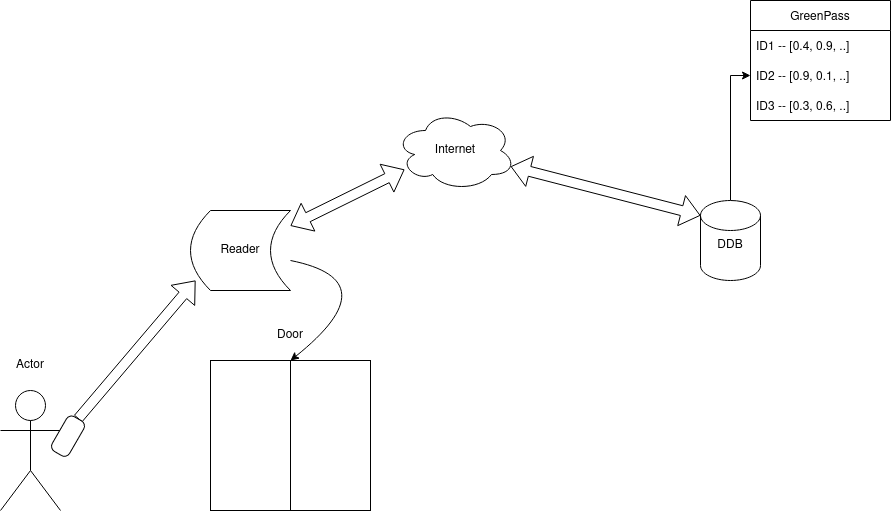
\includegraphics[width=\textwidth,height=\textheight,keepaspectratio]{./Images/Graphic_System.png}
    \label{47_1}
\end{figure}

FARE GRAFICI, DISEGNARE IL SISTEMA, MAGARI EVENTUALI IMPLEMENTAZIONI

TALK ABOUT MECHANISM OF FACE RECOGNITION AND ESTABLISH AN ENTIRE SYSTEM THAT DO THIS WORK (IT CAN BE ENOUGHT ??)


BIBLIOGRAPHY:

https://fossbytes.com/which-smartphone-sensors-how-work/ FOR LIST OF SENSORS IN SMARTPHONES

\end{document}

